The "Center of mass" method of measuring asymmetry is relatively easy to calculate and is more accurate compared to other complex algorithms \cite{Premaladha_2014}.

This algorithm begins by calculating an array of radii from the lesion's center of mass to border for each of 360 degrees. The coordinates for the center of mass are calculated from the sum of all x and y coordinates of pixels within the lesion's border each divided by the sum of pixels.

For each of the 360 radii $r_i$ a score is calculated by comparing the lengths of pairs of radii that are symmetric across $r_i$. If the lengths of the pair of symmetric radii have a difference of less than 10\% then a point is given. The sum of points is the $SFA_i$ (Score For Axis) for $r_i$.

\begin{figure}[H]
    \centering
    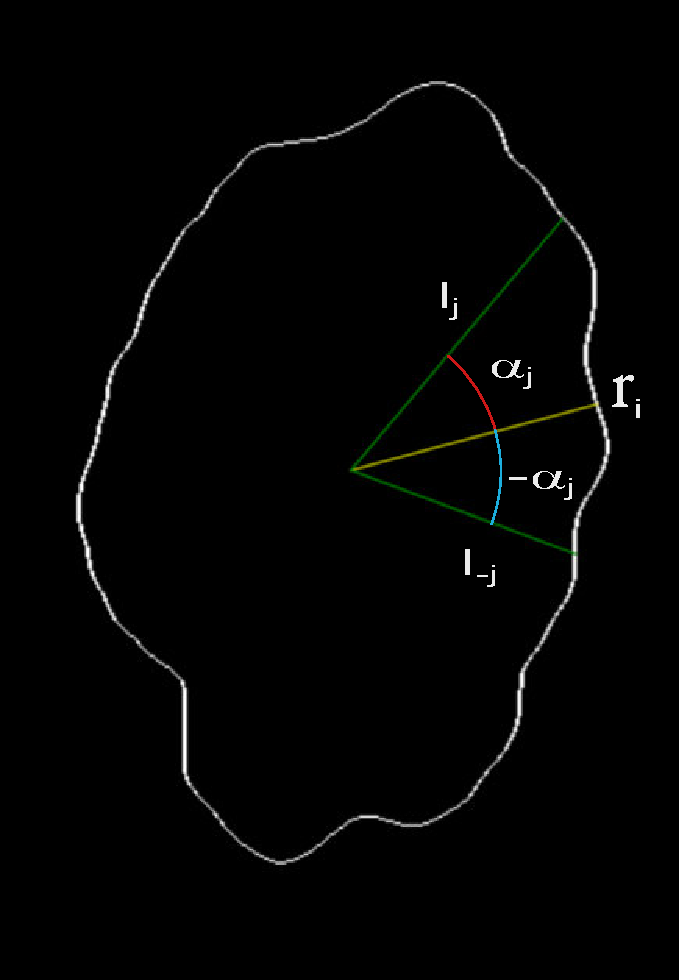
\includegraphics[height=6cm,keepaspectratio]{assets/assymertry/asymmetry_01.pdf}
    \caption{Calculate SFA for $r_i$}
    \label{fig:sfa}
\end{figure}


 The radius with the maximum SFA score is defined as the major axis of symmetry. The SFA of the major axis as well as the perpendicular are stored. The Asymmetry score is evaluated as follows:


\begin{table}[H]
\centering
\small
    \begin{tabular}{ | l | p{3.5cm} | l | p{3.5cm} |}
    \hline
    SFA Results & Description & Asymmetry Score \\ \hline
    \specialcell[t]{major axis $\geq$ 140 \\ minor axis $\geq$ 140} & Symmetric across both axis & 0  \\ \hline
    \specialcell[t]{major axis $\geq$ 140 \\ minor axis $\textless$ 140} & Symmetric across one axis & 1  \\ \hline
    \specialcell[t]{major axis \textless 140 \\ minor axis \textless 140} & Asymmetric & 2  \\ \hline


    \end{tabular}

    \caption{TDS Evaluation\cite{Weigert_2012}}
    \label{fig:tds_eval}

\end{table}